Bár az elektronikusan közölt információk típusa (pl.: rekeszátmérő) nagyban ismert, hogy pontosan melyik elektronikus kontakt, pontosan milyen módon közli az információt, többnyire ismeretlen.
\subsection{Nikon F csatlakozás}
Az F csatlakozáshoz elérhető közösségi információ önmagában nem megbízható, ezért annak valósságát szükséges megerősíteni.
\subsubsection{Ellenőrzés kontroller implementációval}
Abból a feltételezésből kiindulva, hogy az információ helyes, egy kontroller implementáció készül.
Ha ennek használata közben az objektív az elvárt módon viselkedik, akkor az információ helyes.
Hátránya, hogy amennyiben nem helyes az információ, az eszközök károsulhatnak.
\subsubsection{Ellenőrzés kutatási folyamat megismétlésével}
Amennyiben közösségi kísérletek megismétlése során ugyan azok az eredmények érkeznek be, az információ helyes volt.
Ezen felül elvégezhetőek rajta a Z interfészhez ismertetett eljárások is.
Hátránya, hogy hosszadalmas és nem sokkal gyorsabb, mintha teljes információhiány lenne a kiindulási pont.

\subsection{Nikon Z csatlakozás}
Az F csatlakozással szemben a Z csatlakozás elektronikájáról kizárólak feltételezések nyílvánosal.
Ennek értelmében egyfajta fekete doboznak minősül.
%Ennek a rendszernek a feltárására célszerű megközelítés visszafejtéses módszereket alkalmazni. "A visszafejtés itt úgy van definiálva, mint egy bizonyos hardverhez készült specifikációk létrehozása valaki olyan által, aki nem tartozik az eredeti dizájnerek közé, elsősorban egy egyed vagy egyedek gyűjteményének analizálására vagy dimienziózására alapozva."\cite{Reverse_engineering}
%\subsection{Kontaktok szerepeinek azonosítása}
\label{z_elemzes}
Első lépésként a konkrét kontaktok által szállított információk jelentéseit kell meghatározni.
Ehhez először rögzítenünk kell a kontaktok különböző bemenetére adott reakcióját.
Így miközben egy objektív csatlakoztatva van, méréseket végzünk a kapcsolaton.
Fontos a bemeneti és a kimeneti (jelek a kontaktokon) változásokat összepárósítani, mivel így a bemenetek alapján rendezve könnyebben meghatározható, hogy mely adatokért mely csatornák felelnek.
Ezek a dolgozatban később részletesebben is ismertetve lesznek.
\subsubsection{Adatrögzítés}
A rögzítőberendezés nem feltétlenül képes minden kontaktot egyszerre felügyelni.
Ilyenkor ugyanazokkal a beállításokkal meg kell ismételni a tesztet addig, amíg nem lesz tesztelve az összes kontakt az adott beállítással.
A mérőeszköz párhuzamosan van rákötve az adatkapcsolatra annak érdekében, hogy a kommunikáció zavartalanul menjen végbe.
A használt mérőberendezés a \ref{sec:mero_berendezes}-os szekcióban, az adatrögzítés a \ref{sec:naplozas}-es szekcióban kerül bővebb kifejtésre.
\begin{figure}[H]
	\centering
	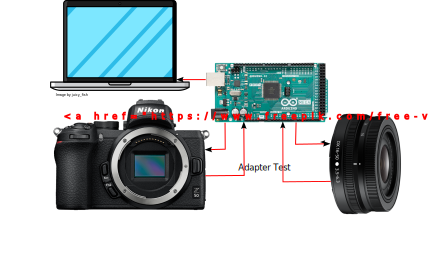
\includegraphics[width=0.9\linewidth]{img/rajz.png}
    \cite{Nikon_Z}\cite{Nikon_Z_16-50}
	\caption{Nikon Z interfész adatrögzítő}
	\label{fig:rogzito}
\end{figure}
\subsubsection{Mintavételezés}
A mintavételezésnek nem sokkal a beállítás megváltozása előtt kell kezdődnie, és a jel végeztével le kell állnia. Ezzel látványosan lehet szemléltetni az értékváltozást, és kinyerhetővé válik a jelváltozás szükséges sebessége, valamint a rögzítés megfelelően időzített leállításával elkerülhető a fölösleges feljegyzések generálása, ezzel csökkentve az adatfeldolgozással töltött időt.
\paragraph{Mintavételezési gyakoriság}
Mivel a jelet rögzítésnél az analízis érdekében analógként kezeljük (nem digitális 1 eseket és nullákat rögzítünk, hanem az elektromos jel fentebb említett tulajdonságainak értékeit rögzítjük), de digitálisan tároljuk, ezért meghatározott időközönként kell mintavételezést végeznünk. Ennek a gyakoriságát a Nyquist-Shannon mintavételezési elmélet alapján határozzuk meg. "A Nyquist elmélet leírja, hogy hogyan lehet mintavételezni egy hullámból úgy, hogy ne vesszen el információ."\cite{por2019nyquist} Eszerint a mintavételezési gyakoriságnak a jel legnagyobb lehetséges frekvenciájának kétszeresének kell lennie (\ref{eq:Nyguist})\cite{por2019nyquist}.

\begin{align}
    f_{minta} \geq 2f_{max}
    \label{eq:Nyguist}
\end{align}	
\cite{por2019nyquist}

Ebből következik, hogy egy mintavételezési gyakoriság alapján meghatározható az a frekvencia, aminél kisebb, vagy azonos frekvenciájú jelek veszteség nélkül visszaállíthatóak (\ref{eq:Nyguist_freq}). Ez a frekvencia a Nyguist frekvencia.

\begin{align}
    f_{Nyguist} = \frac{1}{2}f_{max}
    \label{eq:Nyguist_freq}
\end{align}	
\cite{por2019nyquist}

A maximális frekvencia meghatározásához előbb a mintavételező maximális mintavételezési sebességét használva, interpolációval hozunk létre egy függvényt. Ezt elég minden kontakt esetén egyszer elvégezni, azonban több méréssel, és azok egyesítésével megbízhatóbb eredményt kapunk. Ilyenkor valószínűleg a szükségesnél nagyobb a mintavételezési frekvencia, ezért az interpolációt el lehet végezni. A függvény csúcsai közti idő felhasználásával határozzuk meg az $f_{max}$ frekvenciát. Ezt a (\ref{eq:csucsok}) képlettel kaphatjuk meg. A csúcsokat az g(idő) függvény deriválásával, a deriváltfüggvény zérushelyeinek meghatározásával, és a kapott helyek közül a pozitív függvényértéket felvevők kiválasztásával érdemes elvégezni.

\begin{align}
    f_{max} = \frac{1}{min^{n - 1}_{i = 1}(|t_{i} - t_{i + 1}|)}
    \label{eq:csucsok}
\end{align}	
\small Ahol $n$ a csúcsok száma és $t \in T$ a csúcs rögzítésének ideje.

Egy beállítással több mérést is kell végezni, így csökkentve az esélyét annak, hogy egy vagy több meghibásodásnak köszönhetően rossz konklúzióra jussunk. Az ideális tesztek számát a méréseket végző türelme, és a kapott értékek közti különbségek alapján lehet meghatározni.

\subsubsection{Adatok rendezése}
Hogy könnyebben értelmezhetőek legyenek az összegyűjtött adatok, azokat szűrni és egyesíteni kell. Az alábbi két folyamat elsősorban az összegyűjtött adatok elemzésére szolgál, nem használatosak az adapteren. Ez a módszer nem növeli annyival az adatok pontosságát, hogy az adapteren megérje alkalmazni.
\paragraph{Hibás adatok szűrése statisztikai módszerekkel} A kapott adatokból létrehozunk egy 99\%-os konfidenciaintervallumot, és az azon kívül eső elemeket eltávolítjuk a minták közül úgy, hogy a helyükre a kettő szomszédos érték étlagát írjuk be. Ezáltal a mintavételezési sűrűség nem változik.
\paragraph{Hibás adatok szűrése zajforrás megszüntetésével} Maga a mérőeszköz is képes zajt generálni. Ennek érdekében használjuk a \ref{ADC_noise} kifelytett eljárást.
\paragraph{Zaj szűrése a jel dekompozíciójával} Bizonyos frekvenciákat eltávolítva tisztább, könnyebben elemezhető jelet kapunk. Ehhez egy metódus a \ref{OMP} szekcióban kifejtett módszer.
\paragraph{Összefésülés több mérés esetén}
Mivel az adatrögzítés a minden feljegyzés esetében, a beállításváltozáshoz képest ugyanakkor kezdődik és ér véget, valamint a mintavételezési gyakoriság megegyezik, ezért az egy beállításhoz tartozó adatokat a mérés kezdése óta eltelt idő alapján csoportosíthatjuk. A fenti szűrés elvégzése után a több mintából egyet alakítunk ki úgy, hogy egy ilyen kategóriába tartozó adatoknak az átlagát vesszük, és az így keletkezett feljegyzésből állítjuk vissza az eredeti függvényt. Ez az adapteren nem értelmezhető, mivel csak egy adatfolyammal tud dolgozni, a jelenlegi mérések alapján.
% ide le kellene írni, hogy hogyan kell visszaállítani.

\subsection{Jelek átalakítása}
Az adathalmaz kialakítása után értelmezni kell a kapott függvényeket, és azokból a bemenet alapján kinyerni az adatokat
\subsubsection{Analóg és digitális jelek elkülönítése}
Elektronikus úton két féle képpen lehetséges adatokat továbbítani. Az elektromos jel lehet digitális vagy analóg. A fenti adattranszformációk elvégzése után a függvényt vizualizálva könnyen megállapítható annak típusa következő módon. Amennyiben a függvény értéke két érték között váltakozik, azokat elérve ezeket az értékeket egy bizonyos ideig tartják, akkor ez egy négyzetfüggvény és digitális jelre utal. Amennyiben a jel több értéket is felvesz, valamint hullámossága nagyobb, akkor a jel analóg.

\begin{figure}[H]
	\centering
	\includegraphics[width=0.5\linewidth]{img/oszcilloskóp.png}
    \cite{digital_vs_analog}
	\caption{Analóg (fent) és digitális (lent) az oszcilloskópon}
	\label{fig:oscilloszkop}
\end{figure}

\subsubsection{Analóg jelek transzformálása}
\paragraph{Analóg-Analóg kapcsolat}
Az ilyen típusú jelek pontos jelentését nehéz meghatározni. Ezért amennyiben az adott funkciót mind a Z és az F oldalon analóg jelek látják el, akkor az egyik oldalról kapott mintákon lineáris transzformációt végzünk úgy, hogy a másik oldal interfészének megfeleljen.
\paragraph{Analóg-Digitális kapcsolat}
Ebben az esetben kötelező értelmezni az analóg jelet. Ezt úgy lehet megtenni, hogy az ismert bemenettel asszociáljuk az adatgyűjtés során kapott analóg függvényt. Amennyiben a kapott analóg függvény eléggé hasonlít (a bemenet értékének, annak változásának, valamint a mintafügvény értékének, annak változásának, különbsége határártéken belül van), akkor kimeneti digitális jel az analóg jellel asszociált digitális jelet adja tovább. Amennyiben a jelet digitálisról kell analógra váltani, akkor a kimeneten a digitális jellel asszociált függvényt kell megjelentetni.

\subsubsection{Digitális jelek analizálása és transzformálása}
A digitális jelet elöször demodulárni kell (analógból digitálissá alakítani), miután megállapítottuk a moduláció módját az analóg forrás vizsgálatával. Amennyiben ezt támogatja a mikrokontroller bemenete, annyiban nem szükséges további szoftveres feldolgozást végezni az analóg jelen, máskülönben a demodulációt be kell iktatni a mikroprocesszoron futtatott szoftverbe. Ezt követően a bemenetből és az ipari szabványokból kiindulva dekódolni lehet az adatokat. Azonban ez a legtöbb esetben nem szükséges, mivel a cél a két interfész közti adatmegfeleltetés. Így elég egy hasítótábla segítségével kikeresni digitális jelbemenetnek megfelelő kimeneti adatláncot, és azt továbbküldeni. Amennyiben a két adatlánc közt matematikai összefüggés is leírható, akkor azt érdemes használni a transzformációra, a memóriaigény csökkentése, és a gyorsabb reakció érdekében.